%
% schnittkruemmung.tex -- Schnittkrümmung
%
% (c) 2021 Prof Dr Andreas Müller, OST Ostschweizer Fachhochschule
%
\bgroup
\begin{frame}[t]
\setlength{\abovedisplayskip}{5pt}
\setlength{\belowdisplayskip}{5pt}
\frametitle{Schnittkrümmung}
\begin{center}
\def\pfad{../../buch/chapters/110-kruemmung/images}
\def\links{-4}
\begin{tikzpicture}[>=latex,thick]
\uncover<1>{
	\node at (0,0)
		{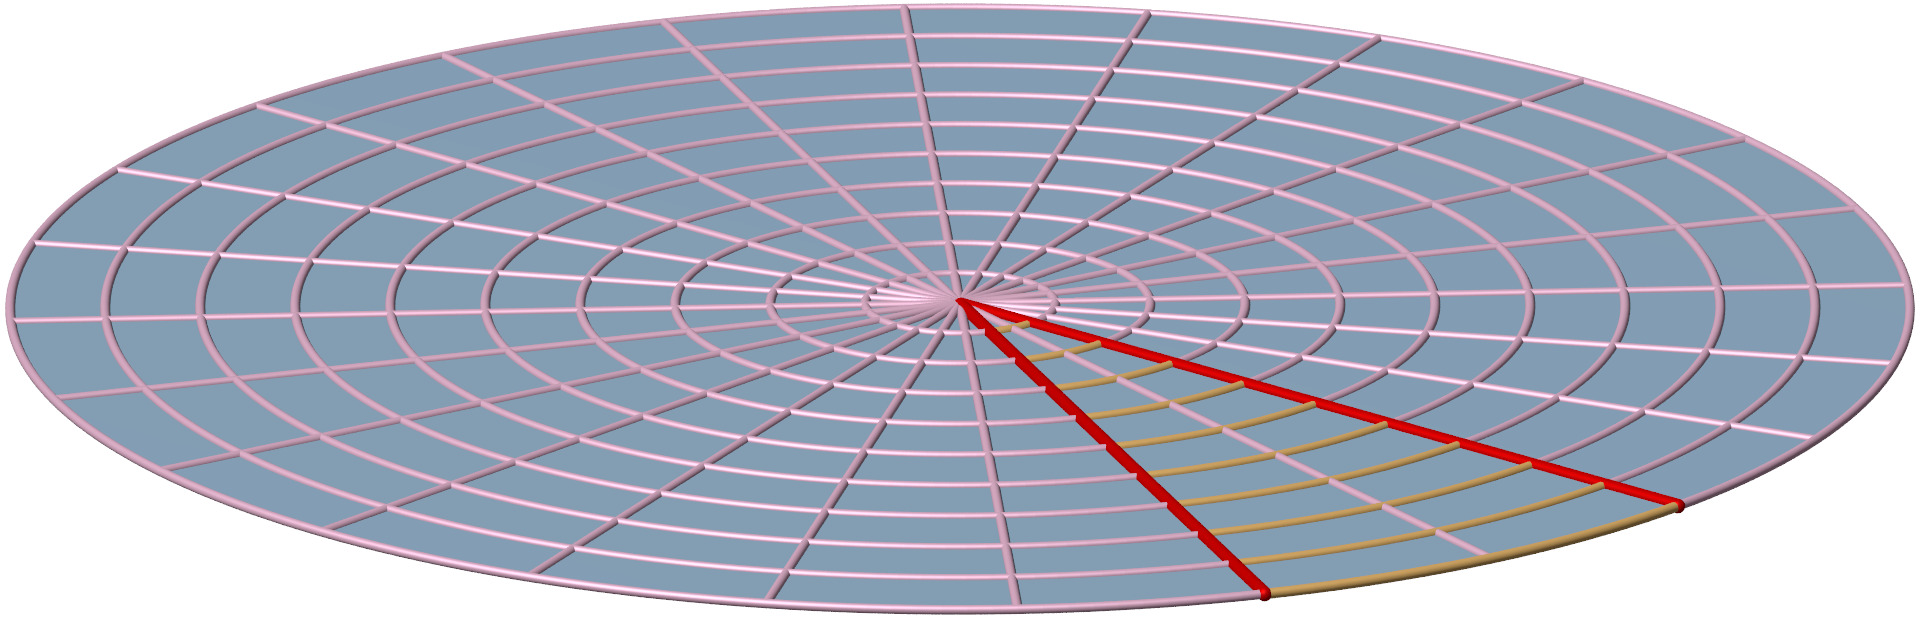
\includegraphics[width=13cm]{\pfad/kruemmung0.jpg}};
	\node at (0,2.4) {$K=0\mathstrut$};
	\node at (\links,-4.3) [right] {Geodätenabstand wächst linear\strut};
}
\uncover<2>{
	\node at (0,-0.68)
		{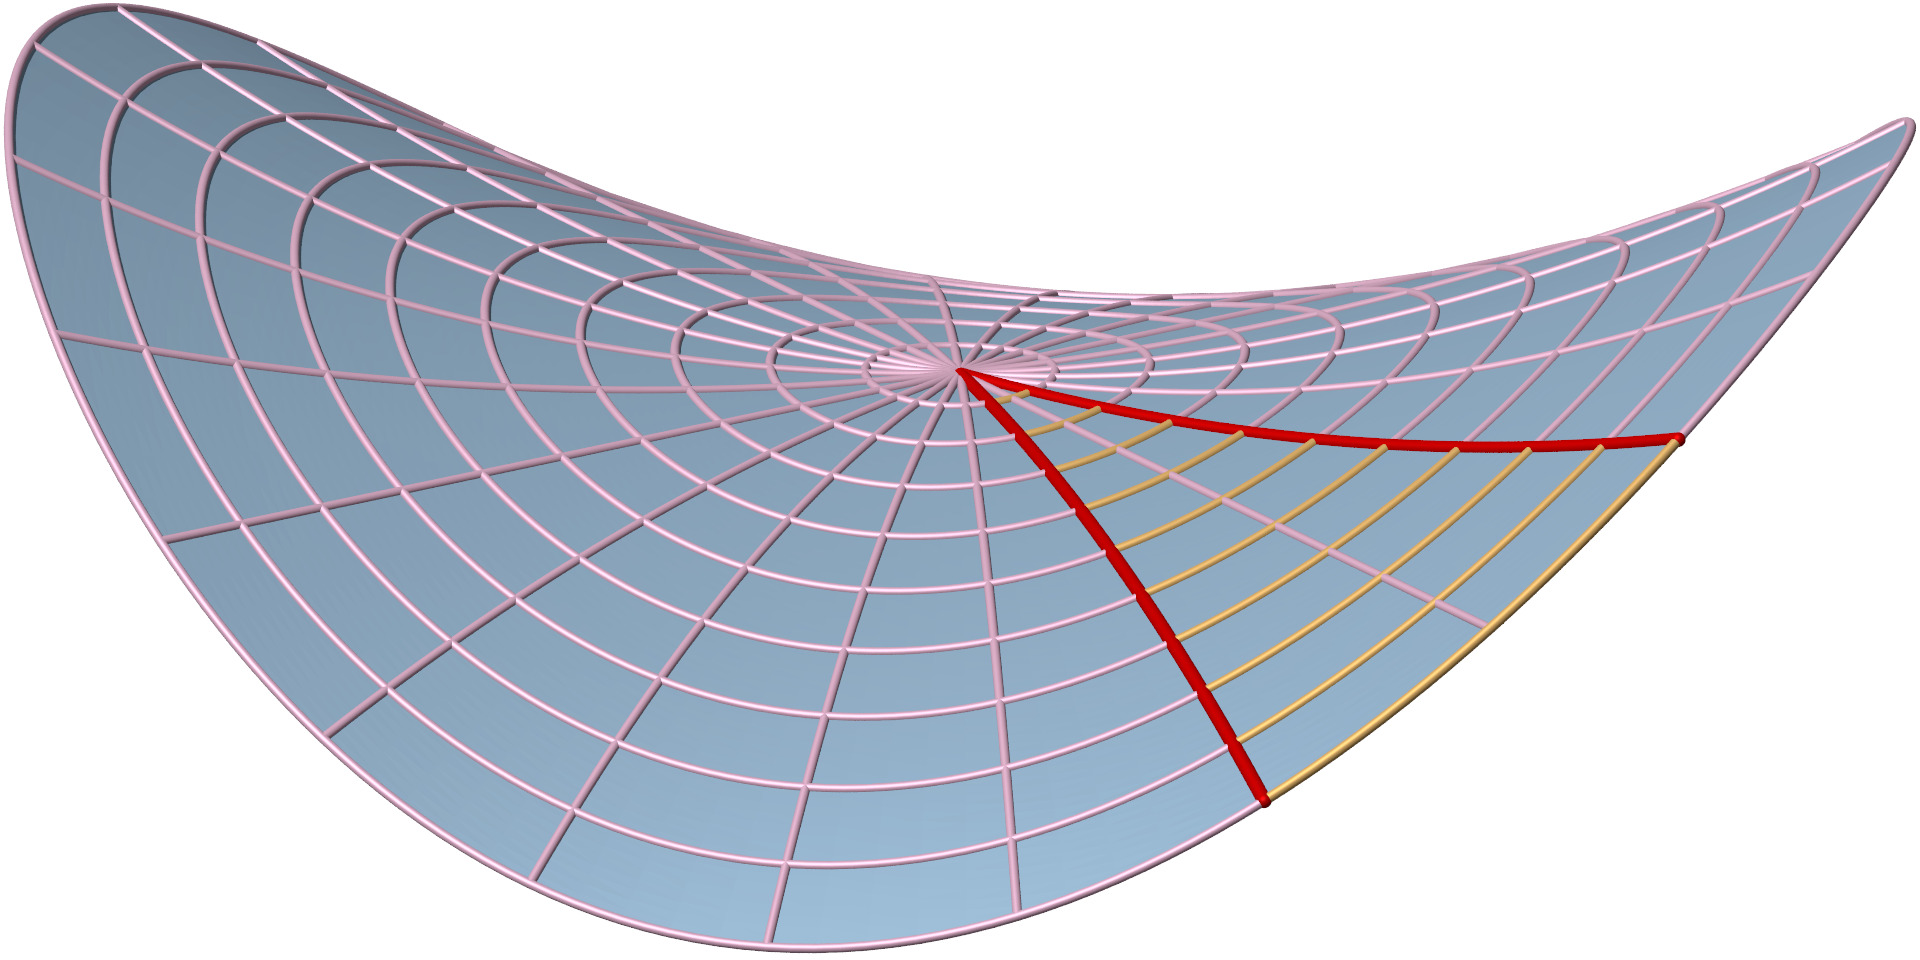
\includegraphics[width=13cm]{\pfad/kruemmungn.jpg}};
	\node at (0,2.4) {$K<0\mathstrut$};
	\node at (\links,-4.3) [right] {Geodätenabstand wächst {\em schneller} als linear\strut};
}
\uncover<3>{
	\node at (0,-1.64)
		{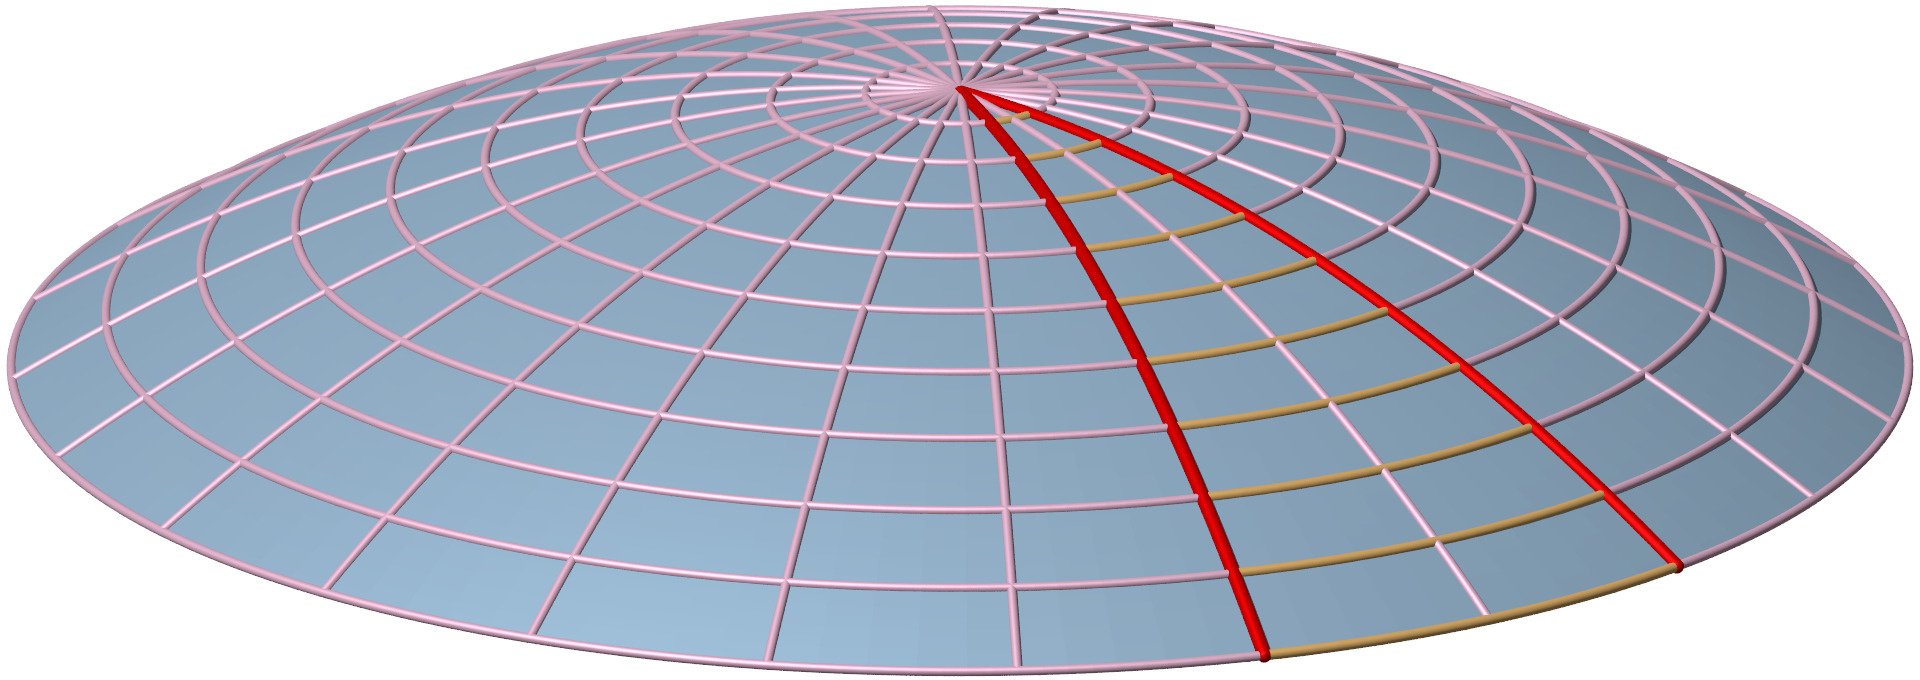
\includegraphics[width=13cm]{\pfad/kruemmungp.jpg}};
	\node at (0,2.4) {$K>0\mathstrut$};
	\node at (\links,-4.3) [right] {Geodätenabstand wächst {\em langsamer} als linear\strut};
}
\end{tikzpicture}
\end{center}
\begin{columns}[t,onlytextwidth]
\begin{column}{0.48\textwidth}
\end{column}
\begin{column}{0.48\textwidth}
\end{column}
\end{columns}
\end{frame}
\egroup
